\chapter{Analysis of related communication protocols}
\label{commprotocols}

% ----------------------------------------------------------------------------
\section{Mix networks}
Mix networks are also known as onion routing or digital mixes and
were invented by David Chaum in 1981.\cite{Chaum:1981:UEM:358549.358563}
\begin{figure}
    \centering
    \caption[Mixes: Packet Flow]{Mixes: Packet Flow\\Image source \url{http://upload.wikimedia.org/wikipedia/en/2/23/Decryption_mix_net.png}}
    \label{mixesflow}
    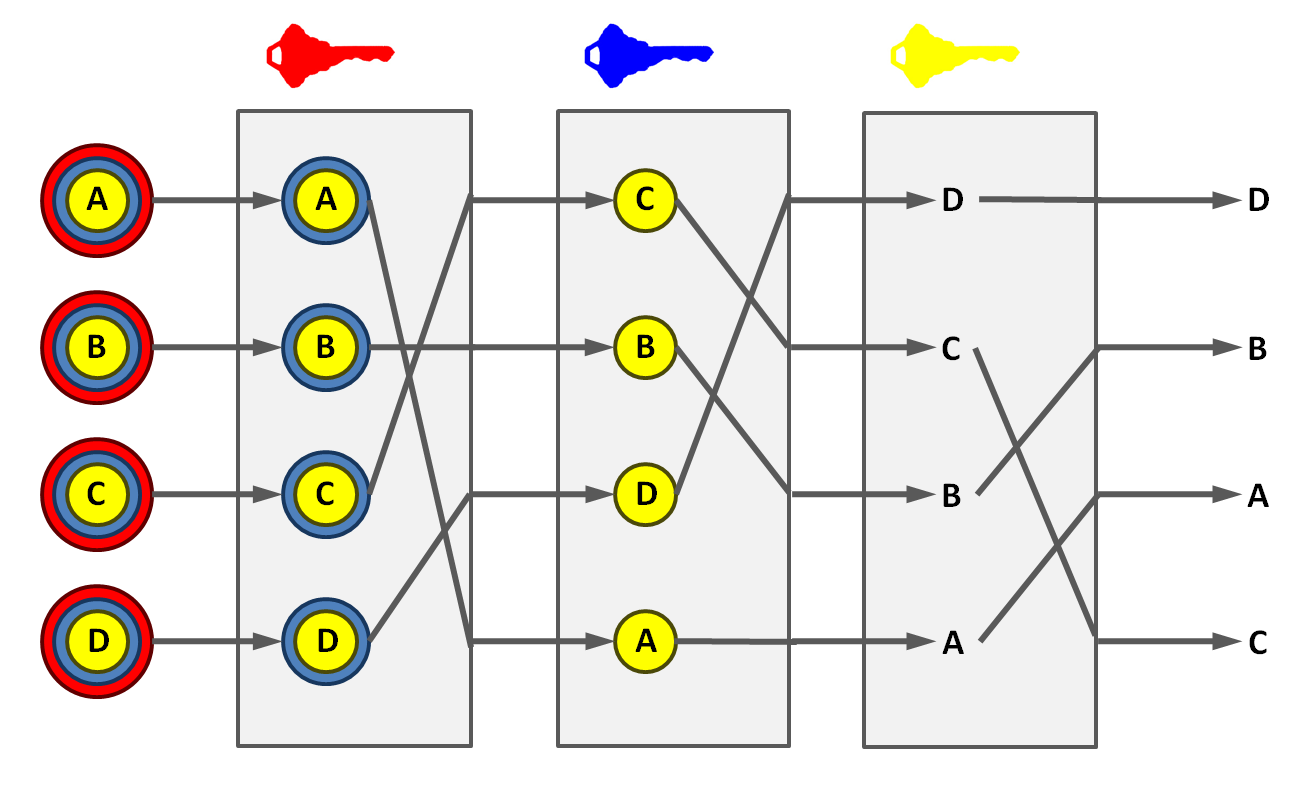
\includegraphics[scale=0.3]{Decryption_mix_net.png}
\end{figure}
The base of Mixes is the multiple encrypted packet that is send through a
number of peers (the mixes) as shown in figure \ref{mixesflow}.
Every peer decrypts the message, which reveals which is the next peer
to send the packet to. Using this method, every peer only knows about
its predecessor and successor. For encryption Public-Key-Cryptography (RSA) is used.
The original approach was focussing on Mixes for e-mail delivery.
% Patent \url{http://patft1.uspto.gov/netacgi/nph-Parser?Sect1=PTO2&Sect2=HITOFF&p=1&u=%2Fnetahtml%2FPTO%2Fsearch-bool.html&r=1&f=G&l=50&co1=AND&d=PTXT&s1=6266704.PN.&OS=PN/6266704&RS=PN/6266704}
% ----------------------------------------------------------------------------
\section{Tor}
The Tor network has been published in 2004
at the 13th USENIX Security Symposium by Roger Dingledine, 
Nick Mathewson and Paul Syverson.\cite{tor}
The idea behind Tor is to provide a general purpose, 
low latency anonymising network stack.
They explicitly do not include application level anonymity
(like stripping user agent information from a http request) and
reason this to leave it up specialised projects.
Tor does (by design) offer no protection against end-to-end attacks
(for instance using traffic analysis) to support low latency applications.
The Tor software provides access to its network via
a SOCKS proxy interface.
Tor does not use the traditional mix approach:
\begin{quote}
Rather than using a single multiply encrypted
data structure (an onion) to lay each circuit, Tor now uses an
incremental or telescoping path-building design, where the
initiator negotiates session keys with each successive hop in
the circuit.\footnote{Quote from \cite{tor}.}
\end{quote}
%\url{http://en.wikipedia.org/wiki/Onion_routing}
% Reply onions have been replaced by a rendezvous system, 
%Generic transport protocol.
%    Separation of “protocol cleaning” from anonymity:

%Onion Routing originally required a separate “application
%proxy” for each supported application protocol—most of
%which were never written, so many applications were never
%supported.
%Tor uses the standard and near-ubiquitous
%SOCKS proxy interface, allowing us to support most
%TCP-based programs without modification. Tor now relies on
%the filtering features of privacy-enhancing application-level
%proxies such as Privoxy [39], without trying to duplicate those
%features itself.
%% No mixing, padding, or traffic shaping (yet): Onion
%% Routing originally called for batching and reordering cells
%% as they arrived, assumed padding between ORs, and in later
%% designs added padding between onion proxie
%% 
%% 
%% Perfect forward secrecy: In the original Onion Routing
%% design, a single hostile node could record traffic and later
%% 
%% ...
%% 
%% 
%% Not secure against end-to-end attacks: Tor does not
%% claim to completely solve end-to-end timing or intersection
%% attacks. Some approaches, such as having users run their own
%% onion routers, may help; see Section 9 for more discussion.
%% 
%% \cite{tor}
% ----------------------------------------------------------------------------
\section{Off-the-Record Messaging (OTR)}
Off-the-Record Messaging (OTR) has been introduced by
Nikita Borisov, Ian Goldberg and Eric Brewer in 2004.\cite{otr}
In contrast to other approaches OTR does not rely on long term
keys as usually used in Public-Key-Cryptography. OTR instead
uses short time keys, to prevent decryption of sniffed messages,
if access to the private key is gained after some time.

Furthermore OTR includes measures to include repudiability, though
provide authentication during a session using
message authentication codes (MAC).
OTR works as a drop in for existing chat programs and offers auto-detection
if the other side is capable of using OTR as well.
%As of OTR 3.1 the protocol supports mutual authentication of users using a shared secret through the socialist millionaire protocol. This feature makes it possible for users to verify the identity of the remote party and avoid a man in the middle attack without the inconvenience of manually comparing public key fingerprints through an outside channel. 
% \url{http://de.wikipedia.org/wiki/Off-the-Record_Messaging}
% ----------------------------------------------------------------------------
\section{Freenet}
Freenet has been published in 2001 by
Ian Clarke , Oskar Sandberg , Brandon Wiley and Theodore W. Hong.\cite{freenet}
Its primary use the anonymous storage (and retrieval) of files.
Freenet is described as follwing:
\begin{quote}
Freenet is free software which lets you anonymously share files, browse and publish "freesites" (web sites accessible only through Freenet) and chat on forums, without fear of censorship. Freenet is decentralised to make it less vulnerable to attack, and if used in "darknet" mode, where users only connect to their friends, is very difficult to detect.\footnote{Quote from \url{https://freenetproject.org/whatis.html}}
\end{quote}
% ----------------------------------------------------------------------------
\section{I2P}
The I2P project, originally Invisible Internet Project, is supposed to be
"`a scalable framework for anonymous communication"'.\cite{i2p} 
It is described on the website as following:
\begin{quote}
I2P initially began in Feb 2003 as a proposed modification to Freenet to allow it to use alternate transports, such as JMS, then grew into its own as an 'anonCommFramework' in April 2003, turning into I2P in July, with code being written in earnest starting in August '03. I2P is currently under development, 
following the roadmap.\footnote{Quote from \url{http://www.i2p2.de/how_intro}.}
\\
...
\\
I2P is a scalable, self organizing, resilient packet switched anonymous network layer, upon which any number of different anonymity or security conscious applications can operate. Each of these applications may make their own anonymity, latency, and throughput tradeoffs without worrying about the proper implementation of a free route mixnet, allowing them to blend their activity with the larger anonymity set of users already running on top of I2P.\footnote{Quote from \url{http://www.i2p2.de/techintro.html}.}
\end{quote}
Although the overall of the impression of the website indicates that it may provide a
reasonable base for anonymous communications, the lack of a central architecture or
design paper makes it hard to judge about it.
%% I2P (initially short for Invisible Internet Project)
%% 
%% I2P is an anonymizing network, offering a simple layer that identity-sensitive applications can use to securely communicate. All data is wrapped with several layers of encryption, and the network is both distributed and dynamic, with no trusted parties.
%% 
%% Many applications are available that interface with I2P, including mail, peer-peer, IRC chat, and others.
%% 
%% 
%%  a low latency, fully distributed, autonomous, scalable, anonymous, resilient, and secure network
%% 
%%   I2P is a low latency mix network, 
%% 
%% 
%% \url{http://en.wikipedia.org/wiki/I2P}
%% 
%% \url{http://www.i2p2.de/_static/images/endToEndEncryption.png}
%% 
%% The first time a client wants to contact another client, they make a query against the fully distributed "network database" - a custom structured distributed hash table (DHT) based off the Kademlia algorithm. This is done to find the other client's inbound tunnels efficiently, but subsequent messages between them usually includes that data so no further network database lookups are required.
%% 
%% This "garlic encryption" lets Alice's router wrap up multiple messages into a single "garlic message",
% ----------------------------------------------------------------------------
\section{RUDP}
Due to the nature of chat messages the use of a stream orientated protocol like
TCP

packet loss: ja
Packet duplicates:
Out of order packets: don't care - no fragmentation
    - probably missing conversation!
    Bit errors: not applicable
    Delay of packets: upper limit (?) 


    - verschieden kaäle:
        - email = sticky, cached, slow
            - tcp = fast, temporarily

            - rudp:
                http://www.javvin.com/protocolRUDP.html
                        rfc908, rfc1151

TCP Reliable transport
UDP
Connectionless
Reliable connectionless\cite{rfc768}

Reliable connectionless\cite{rfc908,rfc1151}

reliable: (up to a maximum number of retransmissions)

In order to gain ensure quality, it extends UDP by adding the following additional features:
Acknowledgment of received packets
Windowing and flow control
Retransmission of lost packets
Overbuffering (Faster than real-time streaming)

% ----------------------------------------------------------------------------
\section{Enet}

\begin{quote}
ENet's purpose is to provide a relatively thin, simple and robust network communication layer on top of UDP (User Datagram Protocol). The primary feature it provides is optional reliable, in-order delivery of packets.

\end{quote}
For unreliable packets, ENet will simply discard the lower sequence number packet if a packet with a higher sequence number has already been delivered. This allows the packets to be dispatched immediately as they arrive, and reduce latency of unreliable packets to an absolute minimum. For reliable packets, if a higher sequence number packet arrives, but the preceding packets in the sequence have not yet arrived, ENet will stall delivery of the higher sequence number packets until its predecessors have arrived.


Reliability

ENet provides optional reliability of packet delivery by ensuring the foreign host acknowledges receipt of all reliable packets. ENet will attempt to resend the packet up to a reasonable amount of times, if no acknowledgement of the packet's receipt happens within a specified timeout. Retry timeouts are progressive and become more lenient with every failed attempt to allow for temporary turbulence in network conditions.

Fragmentation and Reassembly

ENet will send and deliver packets regardless of size. Large packets are fragmented into many smaller packets of suitable size, and reassembled on the foreign host to recover the original packet for delivery. The process is entirely transparent to the developer.

Aggregation

ENet aggregates all protocol commands, including acknowledgements and packet transfer, into larger protocol packets to ensure the proper utilization of the connection and to limit the opportunities for packet loss that might otherwise result in further delivery latency.

Adaptability

ENet provides an in-flight data window for reliable packets to ensure connections are not overwhelmed by volumes of packets. It also provides a static bandwidth allocation mechanism to ensure the total volume of packets sent and received to a host don't exceed the host's capabilities. Further, ENet also provides a dynamic throttle that responds to deviations from normal network connections to rectify various types of network congestion by further limiting the volume of packets sent.

Portability

ENet works on Windows and any other Unix or Unix-like platform providing a BSD sockets interface. The library has a small and stable code base that can easily be extended to support other platforms and integrates easily. ENet makes no assumptions about the underlying platform's endianess or word size.

Freedom

ENet demands no royalties and doesn't carry a viral license that would restrict you in how you might use it in your programs. ENet is licensed under a short-and-sweet MIT-style license, which gives you the freedom to do anything you want with it (well, almost anything).

http://enet.bespin.org/

% ----------------------------------------------------------------------------
%%% High latency:
\section{Remailer}
Besides anonymous networks for generic packet sending, the remailer approach
to send emails anonymiously, have been quite popular.
Projects like Mixmaster\cite{mixmaster}, 
Babel\cite{babel} or Mixminion\cite{mixminion} implement
the Mixes principle\cite{Chaum:1981:UEM:358549.358563}.
%% Low Latency:
%% \section{Anonymizer}
%% The simplest low-latency designs are single-hop proxies
%% such as the Anonymizer [3]: a single trusted server strips
%% the data’s origin before relaying it. These designs are easy to
%% analyze, but users must trust the anonymizing proxy. Concen-
%% trating the traffic to this single point increases the anonymity
%% set (the people a given user is hiding among), but it is vul-
%% nerable if the adversary can observe all traffic entering and
%% leaving the proxy.
%% 
%% \section{Pipenet}
%% PipeNet [5, 12], another low-latency design proposed
%% around the same time as Onion Routing, gave stronger
%% anonymity but allowed a single user to shut down the net-
%% work by not sending. 
% ----------------------------------------------------------------------------
%\section{Further systems}
%Pipenet
%Herbivore
%and
%P5
%go even further, requiring broadcast. 
% ----------------------------------------------------------------------------
\section{Summary}
Report of related communication protocols including strength and weaknesses
